\documentclass[11pt,a4paper]{article}
\usepackage[utf8]{inputenc}
\usepackage[margin=1in]{geometry}
\usepackage{graphicx}
\usepackage{amsmath}
\usepackage{amssymb}
\usepackage{booktabs}
\usepackage{hyperref}
\usepackage{float}
\usepackage{caption}
\usepackage{subcaption}
\usepackage{listings}
\usepackage{xcolor}
\usepackage{tikz}
\usetikzlibrary{shapes,arrows,positioning,fit,backgrounds}

\lstset{
    basicstyle=\ttfamily\small,
    backgroundcolor=\color{gray!10},
    frame=single,
    breaklines=true
}

\title{Hierarchical Hypergraph Neural Network\\for Electromagnetic Particle Simulation}
\author{LAUMeltFlow Project}
\date{\today}

\begin{document}

\maketitle

\begin{abstract}
This report describes a hierarchical hypergraph neural network (H$^2$GNN) architecture for learning electromagnetic interactions between charged particles. Unlike conventional grid-based approaches that discretize fields onto fixed grids, our method treats particles as graph nodes and uses octree voxels as hyperedges to enable efficient multi-scale message passing. The architecture follows a U-Net-like encoder-decoder structure where information flows from particles up through the spatial hierarchy (scatter) and back down to update particle states (gather). Sparse processing ensures that only voxels containing particles are computed, yielding O($N \log N$) complexity.
\end{abstract}

\section{Introduction}

Simulating electromagnetic interactions between charged particles is fundamental to plasma physics, molecular dynamics, and astrophysics. Traditional approaches either compute pairwise forces directly (O($N^2$) complexity) or solve field equations on fixed grids using methods like particle-in-cell (PIC). We explore a neural network approach that learns the particle-to-particle interaction mapping directly.

\subsection{Motivation}

The goal is a learned simulation system where:
\begin{enumerate}
    \item Charged particles exist as nodes with state vectors (position, velocity, acceleration, charge)
    \item An octree partitions space into a hierarchy of voxels
    \item Voxels act as hyperedges connecting particles or child voxels
    \item Message passing propagates information through the hierarchy
    \item Particles update their state based on aggregated local and global information
\end{enumerate}

This approach offers key advantages:
\begin{itemize}
    \item \textbf{Adaptive resolution}: Octree provides fine detail where particles cluster
    \item \textbf{Sparse processing}: Empty voxels are skipped entirely
    \item \textbf{Learned physics}: Network learns interactions from data
    \item \textbf{End-to-end differentiable}: Enables gradient-based optimization
\end{itemize}

\subsection{Physics Background}

For charged particles, the electromagnetic forces are governed by:

\textbf{Electrostatics (Coulomb's law)}:
\begin{equation}
    \mathbf{F}_i = q_i \sum_{j \neq i} \frac{q_j (\mathbf{r}_i - \mathbf{r}_j)}{|\mathbf{r}_i - \mathbf{r}_j|^3}
\end{equation}

\textbf{Magnetostatics (Biot-Savart)}:
\begin{equation}
    \mathbf{B}(\mathbf{r}) = \frac{\mu_0}{4\pi} \sum_j \frac{q_j \mathbf{v}_j \times (\mathbf{r} - \mathbf{r}_j)}{|\mathbf{r} - \mathbf{r}_j|^3}
\end{equation}

\textbf{Lorentz force}:
\begin{equation}
    \mathbf{F} = q(\mathbf{E} + \mathbf{v} \times \mathbf{B})
\end{equation}

The hierarchical structure naturally captures the multi-scale nature of these interactions: nearby particles interact strongly through fine voxels, while distant particles contribute through aggregated effects at coarser levels.

\section{Architecture}

\subsection{Hypergraph Structure}

The architecture is built on a hypergraph where:
\begin{itemize}
    \item \textbf{Nodes}: Charged particles with feature vectors
    \item \textbf{Hyperedges}: Octree voxels at each level of the hierarchy
\end{itemize}

Unlike standard graphs where edges connect exactly two nodes, hyperedges can connect any number of nodes. A leaf voxel connects all particles it contains (0, 1, or more). A parent voxel connects its child voxels.

\begin{figure}[H]
\centering
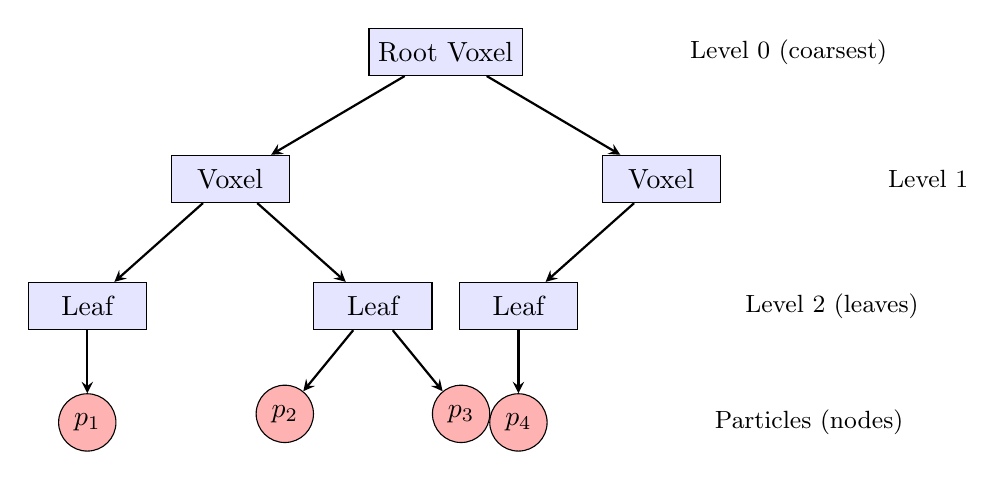
\begin{tikzpicture}[
    level/.style={sibling distance=40mm/#1},
    voxel/.style={rectangle, draw, minimum width=1.5cm, minimum height=0.6cm, fill=blue!10},
    particle/.style={circle, draw, fill=red!30, minimum size=0.5cm},
    arrow/.style={->, >=stealth, thick}
]

% Root
\node[voxel] (root) {Root Voxel};

% Level 1
\node[voxel, below left=1cm and 1cm of root] (v1) {Voxel};
\node[voxel, below right=1cm and 1cm of root] (v2) {Voxel};

% Level 2
\node[voxel, below left=1cm and 0.3cm of v1] (v11) {Leaf};
\node[voxel, below right=1cm and 0.3cm of v1] (v12) {Leaf};
\node[voxel, below left=1cm and 0.3cm of v2] (v21) {Leaf};

% Particles
\node[particle, below=0.8cm of v11] (p1) {$p_1$};
\node[particle, below left=0.8cm and 0.1cm of v12] (p2) {$p_2$};
\node[particle, below right=0.8cm and 0.1cm of v12] (p3) {$p_3$};
\node[particle, below=0.8cm of v21] (p4) {$p_4$};

% Edges
\draw[arrow] (root) -- (v1);
\draw[arrow] (root) -- (v2);
\draw[arrow] (v1) -- (v11);
\draw[arrow] (v1) -- (v12);
\draw[arrow] (v2) -- (v21);
\draw[arrow] (v11) -- (p1);
\draw[arrow] (v12) -- (p2);
\draw[arrow] (v12) -- (p3);
\draw[arrow] (v21) -- (p4);

% Labels
\node[right=2cm of root] {\small Level 0 (coarsest)};
\node[right=2cm of v2] {\small Level 1};
\node[right=2cm of v21] {\small Level 2 (leaves)};
\node[right=2cm of p4] {\small Particles (nodes)};

\end{tikzpicture}
\caption{Hierarchical hypergraph structure. Particles are nodes; octree voxels at each level are hyperedges. Note that voxel v12 contains two particles, illustrating the hyperedge property.}
\label{fig:hypergraph}
\end{figure}

\subsection{Current Configuration}

The current implementation uses:
\begin{itemize}
    \item \textbf{Dimensions}: 2D with quadtree (extensible to 3D octree)
    \item \textbf{Particles}: 10--100 per sample
    \item \textbf{Quadtree depth}: 4 levels (16$\times$16 leaf resolution)
    \item \textbf{Input}: $N$ particles with $(x, y, q)$
    \item \textbf{Output}: $N$ electric field vectors $(E_x, E_y)$
\end{itemize}

\subsection{Node Features}

Each particle node has a feature vector containing:
\begin{itemize}
    \item Position: $(x, y)$ [or $(x, y, z)$ in 3D]
    \item Charge: $q$
    \item Relative position: particle position relative to containing voxel center
    \item (Future) Velocity, acceleration, mass
\end{itemize}

\subsection{Sparse Processing}

A key efficiency feature is that only ``active'' voxels are processed:
\begin{itemize}
    \item A leaf voxel is active if it contains $\geq 1$ particle
    \item A non-leaf voxel is active if it has $\geq 1$ active child
\end{itemize}

Empty branches of the octree are pruned entirely, yielding O($N \log N$) complexity for $N$ particles---similar to Barnes-Hut or Fast Multipole Methods---rather than O($V$) for $V$ total voxels.

\subsection{Encoder (Scatter / Up-Pass)}

Information flows from particles up through the hierarchy:

\begin{enumerate}
    \item \textbf{Relative Position Encoding}: Compute each particle's position relative to its containing voxel center: $\mathbf{r}_{\text{rel}} = \mathbf{r}_p - \mathbf{r}_{\text{voxel}}$
    \item \textbf{Particle $\to$ Hidden}: MLP encodes augmented particle features $(x, y, q, r_{\text{rel},x}, r_{\text{rel},y})$ to hidden state
    \item \textbf{Particle $\to$ Leaf Voxel}: Scatter with \textbf{sum aggregation}:
    \begin{equation}
        \mathbf{h}_{\text{leaf}} = \sum_{p \in \text{leaf}} \mathbf{h}_p
    \end{equation}
    \item \textbf{Child $\to$ Parent}: Sum aggregation of child hidden states
    \item \textbf{Level MLP}: Apply level-specific MLP to aggregated state
    \item \textbf{Repeat} until reaching the root voxel
\end{enumerate}

\textbf{Why sum aggregation?} Mean aggregation loses information about how many particles contributed. Sum preserves particle count information, which is physically meaningful: the total field contribution from a voxel depends on both the charges and the number of particles. Skip connections implicitly carry this count information through the network.

\subsection{Decoder (Gather / Down-Pass)}

Information flows from root back down to particles:

\begin{enumerate}
    \item \textbf{Parent $\to$ Child}: Broadcast parent state to each active child
    \item \textbf{Skip Connection}: Concatenate with encoder state at same level:
    \begin{equation}
        \mathbf{h}'_{\text{child}} = \text{MLP}\left( [\mathbf{h}_{\text{parent}}; \mathbf{h}_{\text{child}}^{\text{enc}}] \right)
    \end{equation}
    \item \textbf{Repeat} until reaching leaf voxels
    \item \textbf{Leaf $\to$ Particle}: Broadcast leaf state to particles (gather)
    \item \textbf{Output}: MLP computes electric field from leaf state and augmented particle features:
    \begin{equation}
        \mathbf{E}_p = \text{MLP}\left( [\mathbf{h}_{\text{leaf}}; x_p, y_p, q_p, r_{\text{rel},x}, r_{\text{rel},y}] \right)
    \end{equation}
\end{enumerate}

\subsection{Skip Connections}

Like a U-Net, each level has skip connections between encoder and decoder:
\begin{itemize}
    \item Encoder state at level $\ell$ is concatenated with decoder input at level $\ell$
    \item Preserves fine-grained spatial information through the bottleneck
    \item Enables gradient flow during training
\end{itemize}

\begin{figure}[H]
\centering
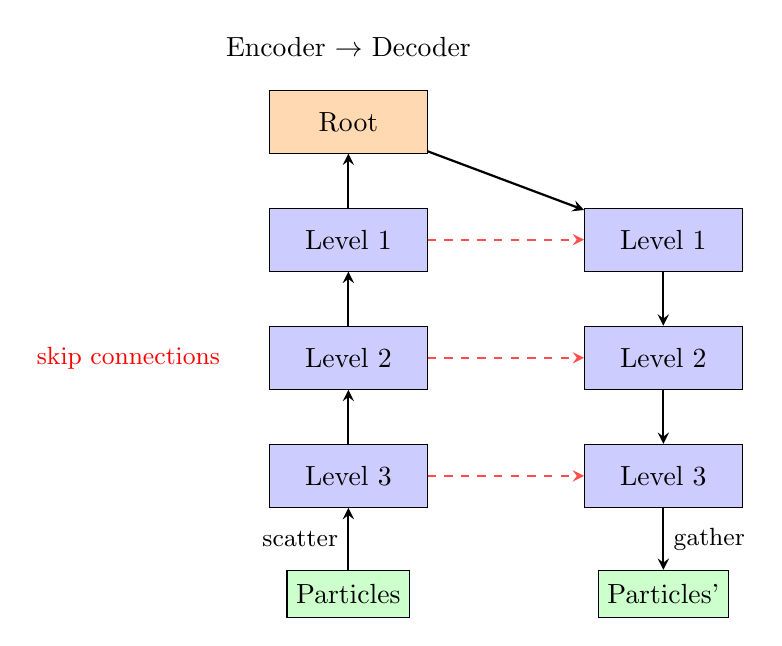
\begin{tikzpicture}[
    block/.style={rectangle, draw, minimum width=2cm, minimum height=0.8cm, fill=blue!20},
    smallblock/.style={rectangle, draw, minimum width=1.5cm, minimum height=0.6cm, fill=green!20},
    arrow/.style={->, >=stealth, thick},
    skip/.style={->, >=stealth, thick, dashed, color=red!70}
]

% Encoder side
\node[smallblock] (p1) at (0,0) {Particles};
\node[block] (e1) at (0,1.5) {Level 3};
\node[block] (e2) at (0,3) {Level 2};
\node[block] (e3) at (0,4.5) {Level 1};
\node[block, fill=orange!30] (root) at (0,6) {Root};

% Decoder side
\node[block] (d3) at (4,4.5) {Level 1};
\node[block] (d2) at (4,3) {Level 2};
\node[block] (d1) at (4,1.5) {Level 3};
\node[smallblock] (p2) at (4,0) {Particles'};

% Encoder arrows
\draw[arrow] (p1) -- node[left] {\small scatter} (e1);
\draw[arrow] (e1) -- (e2);
\draw[arrow] (e2) -- (e3);
\draw[arrow] (e3) -- (root);

% Decoder arrows
\draw[arrow] (root) -- (d3);
\draw[arrow] (d3) -- (d2);
\draw[arrow] (d2) -- (d1);
\draw[arrow] (d1) -- node[right] {\small gather} (p2);

% Skip connections
\draw[skip] (e3) -- (d3);
\draw[skip] (e2) -- (d2);
\draw[skip] (e1) -- (d1);

% Labels
\node[above=0.3cm of root] {Encoder $\rightarrow$ Decoder};
\node[left=0.5cm of e2, red] {\small skip connections};

\end{tikzpicture}
\caption{U-Net-like encoder-decoder structure with skip connections. The encoder scatters particle information up through the octree hierarchy. The decoder gathers global context back down to update particle states.}
\label{fig:unet}
\end{figure}

\section{Comparison with Grid-Based Methods}

\begin{table}[H]
\centering
\begin{tabular}{lll}
\toprule
Aspect & Convolutional U-Net & H$^2$GNN (This Work) \\
\midrule
Input & Fixed grid (field values) & Variable particle set \\
Layers & 2D/3D convolutions & Hypergraph message passing \\
Processing & Dense (all grid cells) & Sparse (active voxels only) \\
Resolution & Fixed grid size & Adaptive octree \\
Output & Field on grid & Particle state updates \\
Complexity & O(grid size) & O($N \log N$) \\
\bottomrule
\end{tabular}
\caption{Comparison between conventional convolutional U-Net and the proposed hierarchical hypergraph approach.}
\label{tab:comparison}
\end{table}

\section{Analytical Reference Implementation}

Before training the neural network, we developed analytical solvers to generate ground truth data and validate the physics.

\subsection{2D Electrostatic Potential}

For a set of point charges, the electrostatic potential in 2D is:
\begin{equation}
    \phi(\mathbf{r}) = -\sum_i q_i \ln|\mathbf{r} - \mathbf{r}_i|
\end{equation}

This satisfies Poisson's equation $\nabla^2 \phi = -\rho/\epsilon_0$.

\subsection{Implementation}

The analytical solver is implemented in \texttt{electrostatic\_unet/electrostatic\_2d.py}:
\begin{itemize}
    \item \texttt{generate\_particles()}: Creates random point charges
    \item \texttt{compute\_potential()}: Computes analytical potential
    \item \texttt{compute\_electric\_field()}: Derives $\mathbf{E} = -\nabla\phi$
\end{itemize}

\subsection{Verification}

Two verification tests confirm correctness:

\subsubsection{Poisson's Equation}
The numerical Laplacian $\nabla^2\phi$ is compared to $-\rho$. Figure~\ref{fig:poisson_verification} shows the localized peaks at particle positions.

\subsubsection{Superposition Principle}
Particles are split into groups $A$ and $B$, verifying:
\begin{equation}
    \phi(A \cup B) = \phi(A) + \phi(B)
\end{equation}
This test passes to machine precision (relative error $< 10^{-13}$).

\begin{figure}[H]
    \centering
    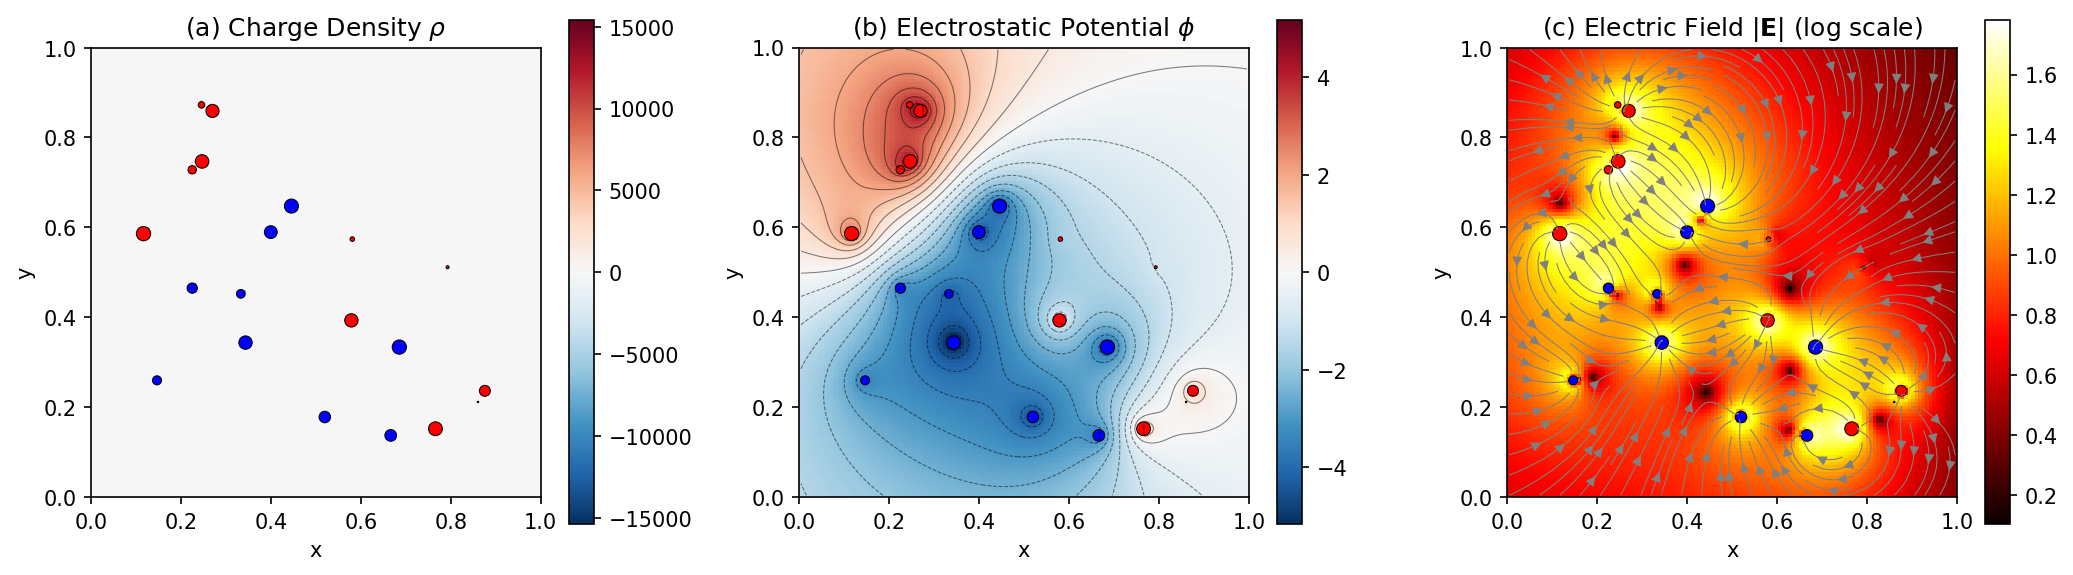
\includegraphics[width=\textwidth]{figures/electrostatic_fields.png}
    \caption{Visualization of 2D electrostatic simulation with 20 random point charges. (a) Charge density. (b) Electrostatic potential with equipotential contours. (c) Electric field magnitude with streamlines.}
    \label{fig:electrostatic_fields}
\end{figure}

\begin{figure}[H]
    \centering
    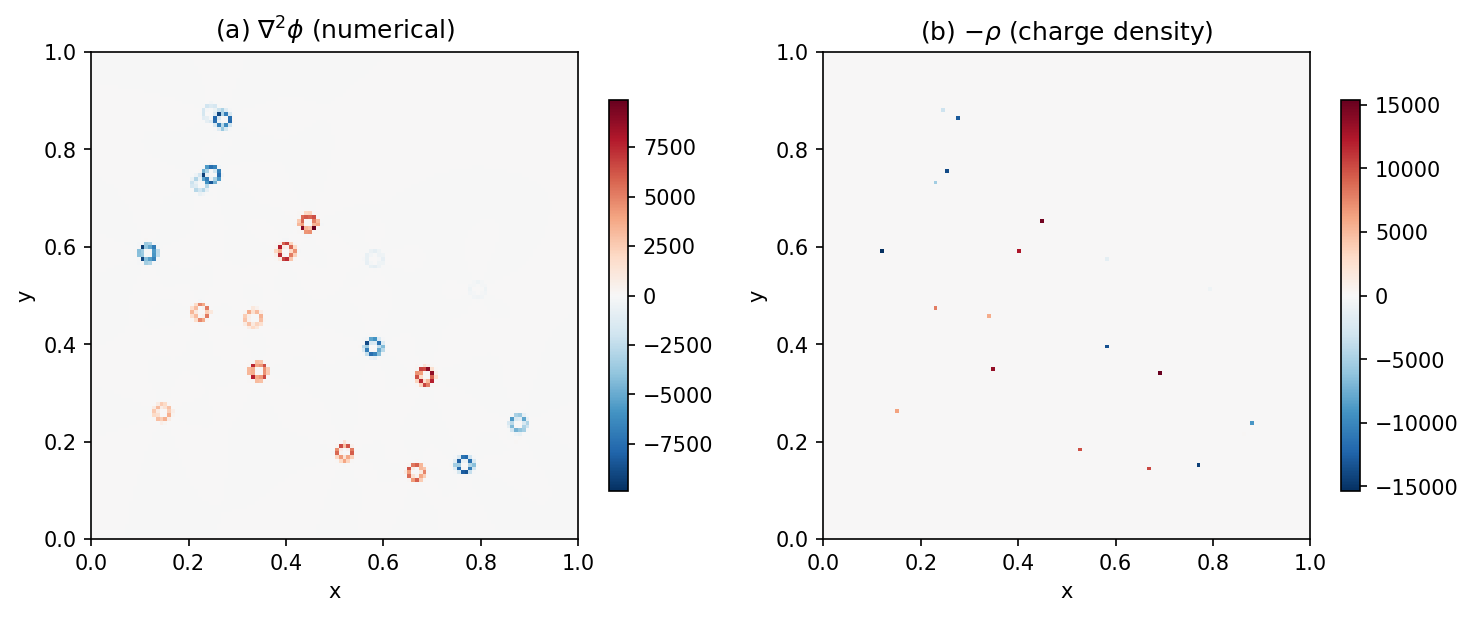
\includegraphics[width=0.85\textwidth]{figures/poisson_verification.png}
    \caption{Verification of Poisson's equation. (a) Numerical Laplacian $\nabla^2\phi$. (b) Negative charge density $-\rho$.}
    \label{fig:poisson_verification}
\end{figure}

\begin{figure}[H]
    \centering
    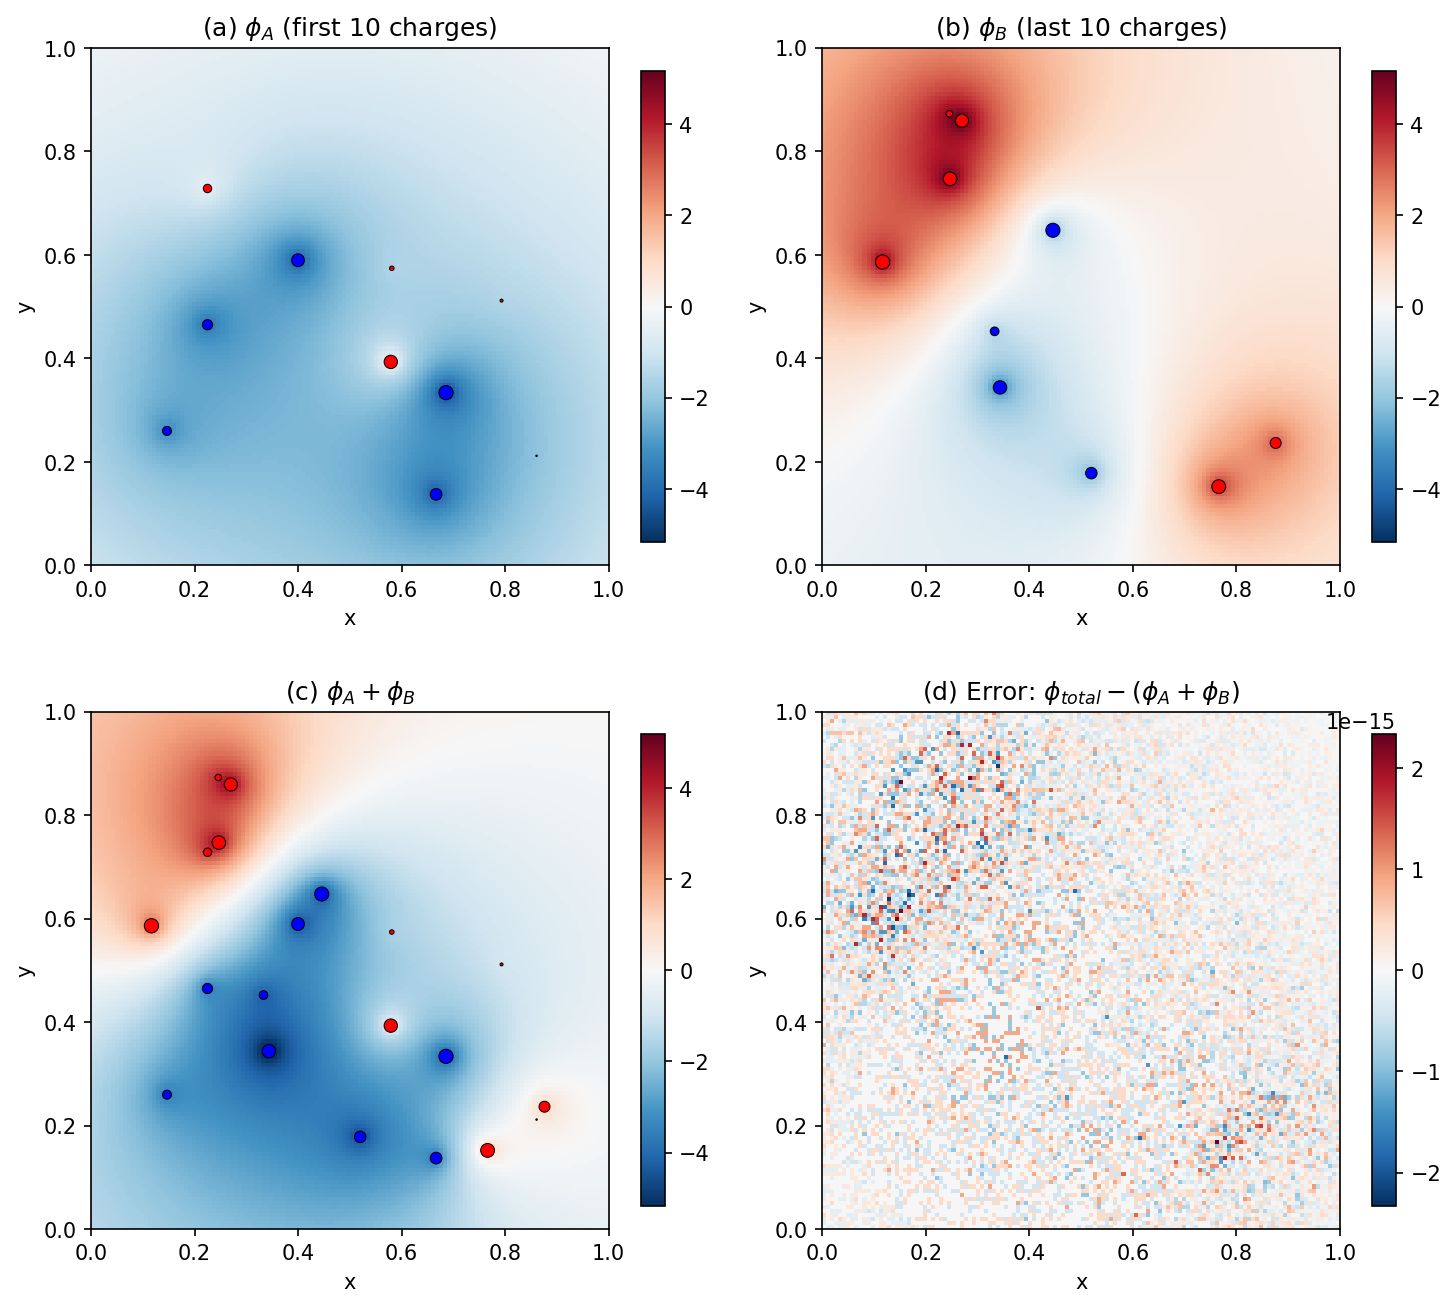
\includegraphics[width=0.85\textwidth]{figures/superposition_test.png}
    \caption{Verification of superposition principle showing machine-precision agreement.}
    \label{fig:superposition}
\end{figure}

\section{Training Data Generation}

Training data is generated using brute-force O($N^2$) Coulomb computation:

\begin{enumerate}
    \item \textbf{Input}: Generate $N$ random particles in $[0, 1]^2$ with charges in $[-1, 1]$
    \item \textbf{Output}: Compute ground truth electric field at each particle using pairwise Coulomb summation
\end{enumerate}

The ground truth electric field at particle $i$ is computed as:
\begin{equation}
    \mathbf{E}_i = \sum_{j \neq i} \frac{q_j (\mathbf{r}_i - \mathbf{r}_j)}{|\mathbf{r}_i - \mathbf{r}_j|^2}
\end{equation}

This is implemented using vectorized operations:
\begin{lstlisting}[language=Python]
# Vectorized 2D Coulomb field - O(N^2) computation
r = positions.unsqueeze(1) - positions.unsqueeze(0)  # (N, N, 2)
r_mag = torch.norm(r, dim=-1)  # (N, N)
E = (charges * r / r_mag**2).sum(dim=1)  # (N, 2)
\end{lstlisting}

\textbf{Key insight}: The ground truth computation is O($N^2$), but the trained network approximates this with O($N \log N$) complexity using the hierarchical quadtree structure---similar to how Barnes-Hut or Fast Multipole Methods work, but with learned rather than analytical approximations.

\begin{table}[H]
\centering
\begin{tabular}{ll}
\toprule
Parameter & Value \\
\midrule
Particles per sample & 10--100 \\
Charge range & $[-1, 1]$ \\
Domain & $[0, 1]^2$ \\
Quadtree depth & 4 levels \\
Training samples & 1,000+ \\
Validation samples & 200+ \\
\bottomrule
\end{tabular}
\caption{Training data generation parameters.}
\label{tab:data_params}
\end{table}

\section{Training}

The training loop proceeds as follows:

\begin{enumerate}
    \item Generate random particle configuration (positions + charges)
    \item Compute ground truth E field using O($N^2$) Coulomb summation
    \item Build quadtree from particle positions
    \item Forward pass through H$^2$GNN $\to$ predicted E field
    \item Compute loss $= \text{MSE}(\mathbf{E}_{\text{pred}}, \mathbf{E}_{\text{true}})$
    \item Backpropagate and update weights
\end{enumerate}

\textbf{Hyperparameters}:
\begin{itemize}
    \item \textbf{Loss}: MSE between predicted and ground truth E field
    \item \textbf{Optimizer}: Adam with learning rate $\sim 10^{-4}$
    \item \textbf{Scheduler}: ReduceLROnPlateau (halve LR on plateau)
    \item \textbf{Hidden dimension}: 64
    \item \textbf{MLP layers}: 2 per level
    \item \textbf{Checkpointing}: Best model and periodic saves
\end{itemize}

\textbf{Goal}: Train the network to approximate the expensive O($N^2$) Coulomb computation using the efficient O($N \log N$) hierarchical structure. Once trained, inference is fast.

\section{Evaluation Metrics}

\begin{enumerate}
    \item \textbf{MSE/RMSE}: Mean squared error on E field prediction
    \item \textbf{MAE}: Mean absolute error
    \item \textbf{Relative Error}: Error normalized by field magnitude: $|\mathbf{E}_{\text{pred}} - \mathbf{E}_{\text{true}}| / |\mathbf{E}_{\text{true}}|$
    \item \textbf{Visualization}: Side-by-side ground truth vs predicted E vectors
    \item \textbf{Scaling}: Test on particle counts outside training distribution
    \item \textbf{Timing}: Compare to O($N^2$) direct computation
\end{enumerate}

\section{Implementation Status}

The following modules have been implemented in \texttt{electrostatic\_unet/}:

\begin{enumerate}
    \item \textbf{quadtree.py}: Sparse quadtree data structure, tracks only active voxels
    \item \textbf{h2gnn.py}: H$^2$GNN model with encoder-decoder, weight sharing per level
    \item \textbf{dataset.py}: Vectorized 2D Coulomb field computation, dataset class
    \item \textbf{train.py}: Training loop with validation, LR scheduling, checkpointing
    \item \textbf{evaluate.py}: Metrics computation, E field visualization, quadtree visualization
\end{enumerate}

\textbf{Quick start}:
\begin{lstlisting}[language=bash]
# Train
python -m electrostatic_unet.train --epochs 100 --n-train 1000

# Evaluate
python -m electrostatic_unet.evaluate --checkpoint checkpoints/h2gnn_best.pt
\end{lstlisting}

\section{Future Extensions}

\begin{itemize}
    \item Adaptive octree refinement based on particle density or gradients
    \item Recurrent/temporal processing for time evolution
    \item Full 3D electromagnetic fields with moving charges
    \item Hybrid methods combining learned and analytical forces
    \item Inverse problems: infer particle properties from trajectories
\end{itemize}

\section{Conclusions}

We have implemented a hierarchical hypergraph neural network (H$^2$GNN) that learns to compute electric fields from charged particle configurations. The key features are:
\begin{itemize}
    \item Particles as nodes with $(x, y, q)$ features plus relative position encoding
    \item Quadtree voxels as hyperedges with weight sharing per level
    \item Sparse processing of only active voxels (O($N \log N$) complexity)
    \item U-Net-like encoder-decoder with skip connections
    \item Sum aggregation to preserve particle count information
    \item Training on O($N^2$) ground truth, inference at O($N \log N$)
\end{itemize}

The architecture is designed to learn efficient approximations to the expensive pairwise Coulomb computation, analogous to how Barnes-Hut and Fast Multipole Methods achieve speedups through hierarchical approximation.

\end{document}
